\scanpage{38}
3. Homomorphisme \(\ell\)-adique associé à une \deleted{\unsure{hom}} famille abélienne de cycles.

Soit \(A\) une V.A., \(Z\in A^i_{\mathrm{alb}}(X\times A)\), d'où
\[
\deleted{\unsure{\varphi=}}u_Z:A(k)\longrightarrow A^i_{\mathrm{alb}}(X)
\]
mais aussi
\[
a({}^tZ):H^{2(n-i)+1}(X)(n-i)\longrightarrow H^1(A)
\]
(coefficients \(\ell\)-adiques \(\deleted{\unsure{\mathbb Q}}\mathbb Z_\ell\)). Je dis que mod. torsion (i.e. à coefficients \(\mathbb Q_\ell\)!) cet homomorphisme ne dépend que de \(u_Z\), pas de \(Z\), \deleted{\unsure{donc}} et de façon précise que

\figure{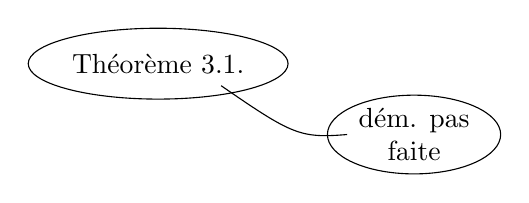
\begin{tikzpicture}[x=1cm,y=1cm]
\node at (0,0) {\uline{Théorème} 3.1.};\draw (0,0) ellipse (1.65 and .45);
\draw (.8,-.28) .. controls (1.7,-.9) and (1.8,-.95) .. (2.4,-.9);
\draw (3.25,-.9) ellipse (1.1 and .5);\node[align=center] at (3.25,-.9) {dém. pas\\faite};
\end{tikzpicture}}
\diagram{\begin{tikzcd}[ampersand replacement=\&,column sep=large,execute at end picture={\node at ([xshift=2mm]hyp.east) {$\unsure{<|\Longleftarrow}$};}]
|[alias=hyp]|u_Z=0\arrow[r,Rightarrow,"?"]\&a({}^tZ):H^{(n-i)+1}\mathbin{-}H^1\text{ est nul}
\end{tikzcd}}
\margin{?\quad A-t-on une réciproque}

\uline{Démonstration}. Choisissons une ``courbe ample'' \(C\) sur \(A\), \deleted{\unsure{d'ici alors}} d'où \(C\longrightarrow A\) induit
\diagram{\begin{tikzcd}[ampersand replacement=\&]
\deleted{C\times X\mathbin{-}}\inserted{X\times C}\arrow[r]\&\deleted{A_C\longrightarrow A}\inserted{X\times A}
\end{tikzcd}}
d'où \(Z'\in A^i_{\mathrm{alb}}(C\times X)\) et pr conséquent
\[
u_{Z'}:C(k)\longrightarrow A^i_{\mathrm{alb}}(X)
\]
\[
a({}^tZ'):H^{2(n-i)+\unsure{3|1}}\deleted{(\unsure{X})}(n-i)\mathbin{-}H^1(C)
\]
et comme \(H^1(A)\mathbin{-}H^1(C)\) est injectif, \(C(k)\mathbin{-}A(k)\) surjectif, on a
\mspage{37}
